
\section*{Abstract}
In recent years, both the scientific community and policy makers are gaining
confidence in the formulation and use of mathematical models in ecological 
studies. We are thus seeing a flourishing of more elaborate and complex models, 
and the questions related to the efficient, systematic and error-proof 
exploration of parameter spaces are of great importance to better understand, 
estimate confidences and make use of the output from these models. In this work,
we investigate some of the relevant questions related to parameter space
exploration, in particular using the technique known as Latin Hypercube 
Sampling and focusing in qualitative and quantitative output analysis.
We present improvements to the methods discussed, and 
assess how are these questions being currently addressed in the literature.
Full working examples are given in the R language, included at the appendix.

NOTA: V\~ ao ser incluidas muito mais refs posteriormente!

%TODO Incluir uma {\em Key references:}  a cada sessao!
%TODO: Toy Model morfometrico, estoque de carbono??
%TODO: Ca\c car todas as refs da Marino08
%TODO: Gente grande na area: Saltelli, Helton, Iman, McKay, Sobol, Conover. LER todos eles

\section{Introduction}\label{Introduction}
There is a growing trend in the use of mathematical modelling tools in the
study of many areas of the biological sciences. The use of models is essencial
as they present an opportunity to address questions that are impossible or
impractical to answer in either in purely theoretical analyses or in field 
or laboratory experiments, and to identify the most important proccesses which
should then be investigated by experiments. Of particular interest are the 
Individual Based
Models (IBM), which represent individuals that move and interact in space,
according to some decision-making rules. 
These models permit a great level of detail and realism to be included,
as well as linking multiple levels of complexity in a system.

On the other hand, more realistic models employ a vast selection of input
parameters, from temperature and rainfall to metabolic and encounter rates,
which may be difficult to accurately measure. While variations in some of those
parameters will have negligible impact on the model output, other parameters
may profoundly impact the validity of a model's predictions, and it may be
impossible to determine {\em a priori} which are the most important parameters.
In theory, this could be done by evaluating the model at all possible 
combinations of parameters, however this would require a prohibitive number of
model runs, specially considering that a single run of those models may take
days to complete. Our challenge then consists in providing the best estimates
for the importance of the several parameters, requiring the least number of
model runs.

The disciplines of uncertainty and sensivity analysis have been developed in
the context of the physical sciences and engineering, and have been greatly
developed in the 1980 and 1990 decades by researches such as Saltelli, 
Helton, Iman, Conovoer, Sobol' and McKay. More recently, these analyses
have been 
successfully applied to biological models, in order to explore the possible 
outcomes from the model output, estimate their
probability distribution and the dependency of the output 
on different combinations of parameters, and to assess which parameters 
require more experimental effort in order to be more confidently estimated. 
This kind of parameter space exploration is considered a fundamental step
prior to using the model in management decisions \cite{Bart95}. 

One approach to the parameter space exploration, which will be described here,
is to generate samples from the parameter space, run the model with these 
samples, and analyse the qualitative or quantitative differences in the
model output. Section \ref{Sampling} will present the sampling techniques,
with empashis on the Latin Hypercube method, while sections \ref{QualAnal} and
\ref{QuantAnal} will deal with qualitative and quantitative analyses, 
respectively. Then, we briefly review some relevant research papers which
have used such techniques in the exploration of ecological models in section
\ref{Studies}, and present a full working example of the sampling and analysis
in the Appendixes.

\subsection{Parameter spaces}\label{ps}
In order to better pose our questions, we need first to have a precise 
definition of what is the parameter space (or PS for short)
of our models, and to distinguish the general use of this expression by the
statistical and the modeling community \cite{Ross90}.

\begin{verbatim}
TODO
\end{verbatim}

Also, it should be mentioned that the parameter space may be constrained or
unconstrained. This will have an impact on some of the available sampling 
and analysis techniques.

For example, let us consider the space of all triangles with one fixed side. We
will use as parameters the angles of the triangle (fig. \ref{fig:triangle}),
$a_1$, $a_2$ and $a_3$. As the sum of the angles is $180 ^o$, we can fix 
$a_3 = 180 ^o - a_1 - a_2$. In addition, the sum of $a_1 + a_2$ must not 
exceed $180 ^o$. The condition

\begin{equation}
	a_1 + a_2 \leq 180 ^o
	\label{samplecond}
\end{equation}

is called a constraint, and limits the values that the parameter vector
may assume. We will return to questions related to constrained parameter
spaces in section \ref{ext}.

\begin{figure}[htbp]
	\begin{center}
		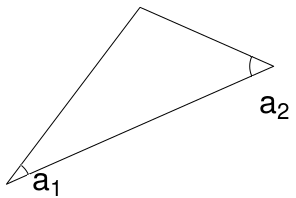
\includegraphics[width=200 pt]{fig/figTriangle.png}
	\end{center}
	\caption{A sample triangle with the angles $a_1$ and $a_2$ highlighted.}
	\label{fig:triangle}
\end{figure}

\subsection{Problems in parameter space exploration}\label{PSE}
Next, we turn our attention to the kind of problems we might want to address
with the exploration of the parameter space. First, the simplest case is asking
``is there a region of my parameter space where condition X holds?'' This 
condition might be, for example, the extinction or coexistance of species, 
some pattern of distribution or abundance of species. We also might be 
interested in mapping where are these regions. In complex models, where several 
different regions might exist where the qualitative results of the models are 
very different, we may ask how many of these regions are there, as well as map
the frontiers between them. We will explore some tools that deal with these 
qualitative problems in section \ref{QualAnal}.

Another class of problems arises when the model produces some quantitative 
response, and we are interessed in determining the dependency of this response 
to the input parameters. For example, when modeling the dynamics of a 
population, we might want to know how the final population varies with each 
of the input parameters. In this context of quantitative analysis, the 
questions are divided in two classes: first, how much the variation of the 
input parameters is translated into the total variation of the results, 
which is the topic of uncertainty analysis, 
and second, how much of the variation in the results can be ascribed to the 
variation of each individual parameter, which is the topic of sensitivity 
analysis \cite{Helton03, Helton05}. We will present the techniques and results
from both uncertainty and sensitivity analysis in section \ref{QuantAnal}.

All these problems may be formulated in a general way, defining some response 
from the model $\bu{Y}$ as a function of the input parameter vector $\bu{x}$:

\begin{equation}
	\bu{Y} = \bu{f}(\bu{x})
	\label{genmodel}
\end{equation}

In the equation \ref{genmodel}, all the quantities are vectors, indicated by
the boldface. Here, $\bu{x} = [ x_1,x_2,\dots,x_m ]$ represent the parameters
to the model $\bu{f}$, and $\bu{Y} = [ y_1,y_2,\dots,y_n ]$ represent the some
quantitative responses from the model. In some sections, we will discuss the
response as a single value $y$, without loss of generality.

Each of the input parameters $x_i$ is associated with a probability distribution
$D_i(x)$, which represent our degree of knowledge about the values that $x_i$ may
assume (see figure \ref{fig:Di} for examples).

\begin{verbatim}
Conseguir dados reais para gerar Dis
\end{verbatim}

\begin{figure}[htpb]
	\begin{center}
	
\includegraphics{capitulo1-Di}
	\end{center}
	\caption{Four different possible origins from $D_i$ *TODO* melhorar explicacao}
	\label{fig:Di}
\end{figure}

\section{Sampling Techniques}\label{Sampling}
There are several strategies that can be used to choose the samples from the
parameter space that will be used as input to our model of interest. Here,
we will present some of them, along with their limitations, to justify our 
choice for the Latin Hypercube Sampling, which we will describe in section
\ref{LHS}.

One way of exploring the parameter space is to choose a number of possible 
values for each parameter, and run the model for every combination of those 
values. This is called full parameter space exploration, as done 
in \cite{Turchin97}, and altough it 
possesses many advantages, it may become very costly in terms of computer time. 
In addition, the number of possible combinations increases exponentially with 
the number of parameter dimensions considered.

To circumvent the exponential increase in the number of samples, it is usual
to explore the parameter space in the following fashion: holding all but one
parameter constant, we analyse how the output of a model is affected by one
parameter dimension at a time (as done in \cite{Yang08}). This kind of analysis,
called individual parameter perturbance,
is, however, limited by the fact that the combinations of changed parameters 
may give rise to complex and unexpected behaviours. 

Another viable option would be to
chose $N$ random samples from the entire space, in order to analyse both
the effect of each parameter and the combined effect of changing any
combined number of parameters. This sampling scheme is called random 
sampling, or Monte Carlo sampling,
and has been applied to many biological models \cite{Letcher96}.

Stratified sampling strategies, which are a special case of Monte 
Carlo sampling, consist in strategies for chosing these random samples while,
at the same, making sure that every subdivision (or {\em strata}) of
the distribution is well represented.
As shown on \cite{McKay79}, the estimatives of the statistical properties (such
as the mean or the variance) of the model output are better represented by 
stratified random sampling than by simple random sampling
(see figure \ref{fig:SamplingMethods} for examples). As we shall see in the
next session, the Latin Hypercube sampling is a practical and easy to understand
stratified sampling strategy.

\begin{figure}[htbp]
	\begin{center}
\includegraphics{capitulo1-SamplingMethods}
	\end{center}
	\caption{Illustration of four sampling methods. While the
	full parameter space exploration is clearly representative
	of the whole space, it requires a very large number of samples.
	The individual parameter perturbation chooses samples by
	holding one parameter constant and varying the other, and
	clearly cannot take into account interactions between 
	parameters. The random sampling uses information about the
	whole parameter space with a small number of samples, but
	can oversample some regions while undersampling others. The
	Latin Hypercube (section \ref {LHS}) samples all the 
	intervals with equal intensity.}
	\label{fig:SamplingMethods}
\end{figure}

\subsection{Latin Hypercube: Definition and use}\label{LHS}
In this section, we describe the Latin Hypercube Sampling, and show how it can
be used to efficiently solve the questions posed in section \ref{Introduction}.
We also
discuss what are the available methods for obtaining the LHS. 

Firstly, let us define, in the context of statistical sampling, what is a 
Latin Square:
\begin{definition}
If we divide each side in a square in $N$ intervals, and then take samples
from the square, the resulting square will be called
Latin if and only if there is exactly one sample in each row and each column.
\end{definition}

A Latin Hypercube is simply the generalization of the Latin
Square to an arbitrary number of dimensions $m$. 
From these definitions, it is clear that the number of samples is fixed as $N$
We will show how to estimate the optimal $N$ in section \ref{TDCC}, but for
now it is 
relevant to note that $N$ does not depend on the number of parameters considered.

We will now construct the Latin Hypercube. Let's fix our attention in one parameter
dimension $i$ of the parameter space.
The first step we should take is to divide the range of $x_i$
in $N$ equally probable intervals. In order to do so, we will turn our attention
to the probability distribution of $x_i$, defined on section \ref{ps} as $D_i$.
Recall that this probability distribution must be chosen in a way that represents our
current understanding of the biology of the given system. This function might
be estimated by an expert in the field, it might represent a data set from
field or laboratory work, or in some cases it may be simply the broadest
possible set of parameters, in some cases where the actual values are unknown
or experiments are unfeasible (see fig. \ref{Di}). 

In possession of the distribution function $D_i$, we must sample one point
from each equally probable interval. There are two approaches used here:
it is possible to choose a random value from within the interval (as proposed
by \cite{McKay79}), or instead, we can use the midpoint from each interval 
\cite{Huntington98}. We will use the second approach here.

%TODO Precisa de mais revisao aqui??
The integral of the distribution function is called the cummulative distribution
function $F_i(x)$. This function relates the values $x$ that the parameter may assume
with the probability $p$ that the parameter is less than or equal to $x$.
We will refer to the inverse of the cummulative distribution function, $F_i^{-1}$,
as the quantile function of the parameter $x_i$, as it associates every probability
value $p$ in the range $(0,1)$ to the value $x$ such that $P(x_i \leq x) = p$.
We divide the range $(0,1)$ in $N$ intervals of size $1/N$, and use this quantile
function to determine the $x$ values as the midpoints of each interval. 
Summarizing, we take the $N$ points, represented as $x_{i,k}$, $k \in [1,N]$, 
from the inverse cummulative distribution $F_i^{-1}(x)$ as:

\begin{equation}
	x_{i,k} = F_i^{-1}\left( \frac{k-0.5}{N}\right)
	\label{inverseCDF}
\end{equation}

%After repeating this procedure with the $m$ parameter dimensions,
%we could define the points from our parameter space by associating the coordinates
%as $\bu{x_1} = [ x_{11}, x_{21}, \cdots x_{m1} ]$, 
%$\bu{x_2} = [ x_{21}, x_{22}, \cdots, x_{m2} ]$. 

%However, by doing this, we would be pairing the smallest values from all dimensions\ldots


\begin{figure}[htpb]
	\begin{center}
\includegraphics{capitulo1-Samples}
	\end{center}
	\caption{Sample normal probability distribution, with 5 samples 
	collected and shuffled. Note that the first sample correspond to the 
	second interval, the second sample correspond to the fourth interval,
	and so on.}
	\label{fig:Samples}
\end{figure}

The samples from each dimension are subsequently shuffled, to randomize
the order in which each value will be used
%so the first position
%in the parameter vector $\bu{x}$ might correspond to the third interval from the
%first dimension, the twelfth interval from the second dimension, and so on 
(see example on figure \ref{fig:Samples}).
As the samples come from the distributions $D_i$, and are only reordered, their
(marginal) distribution 
will remain that of $D_i$. However, the joint distribution
of the parameters is still not well defined. In particular, this simple shuffling
may result in some of the parameters to be positively or negatively correlated with
each others, which might be undesirable. Some techniques have been developed to
eliminate these correlation terms or to impose different correlations between the
variables, and will be presented on section \ref{ext}.

It should be noted that, in the mathematical literature, it is usual to refer 
to a somewhat different object as a Latin Square: this would be a square whose 
sides are divided in $N$ intervals, and is filled with $N$ different symbols, 
such that for each row and column there is exactly one occurrence of each 
symbol. The figure \ref{fig:glassLS} shows an example of one ``full'' Latin 
Square.

\begin{figure}[htpb]
	\begin{center}
		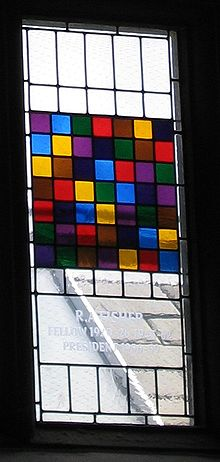
\includegraphics[width=200 pt]{fig/glassLS.png}
	\end{center}
	\caption{A stained glass window at the Caius College, Cambridge, 
	showing a full Latin Square. Notice how there is only one occurence 
	of each color in each row and in each column.}
	\label{fig:glassLS}
\end{figure}

\subsection{Algorithms and extensions}\label{ext}
As described above, the LH sampling generates an uniform distribution of samples 
in each parametric dimension. However, there is no guarantee that the correlation 
between two or more parameters will be zero, and the classical algorithm
from McKay \cite{McKay79} usually produces correlations as high as 0.3 between
pairs of factors, which can difficult or even compromise further analyses. In this
section, we will present one algorithm designed to take into
account the correlation between the parameter variables \cite{Huntington98}, using
a single-switch-optimized sample reordering scheme. 
We will present the general case of prescribing a correlation matrix, and will 
also present results for the trivial case of zero correlation terms. Other
methods have been proposed to address this problem \cite{Ye98, Steinberg06, Florian92}, 
including methods that deal with higher-order correlation terms \cite{Tang98}
using orthogonal designs. These methods, however, impose severe restrictions 
on the number of samples that must be chosen.

In order to obtain the samples with prescribed correlation terms, we define the 
desired $m \times m$ correlation matrix between the variables, in which 
$C_{i,j}^*$ stands for the correlation between $x_i$ and $x_j$.

The next step is done iteratively for each parameter dimension, starting with the second one. Suppose that the method has already been applied to $i=1,2,....,l-1$, 
and we will apply it to $i=l$. The square sum of the errors in the correlations 
between $x_l$ and the anterior parameters is given by

\begin{equation}
	E = \sum_{k=1}^{l-1} \left( C_{l, k} - C_{l,k}^* \right) ^2
	\label{Error}
\end{equation}

Afterwards, we calculate, for each pair of values sampled from the parameter 
dimension $l$, what would be the error in the correlation if they were switched.
The pair that corresponds to the greater error reduction is then switched, and
the procedure is repeated iteratevely until the error is acceptably small.

Here, we also consider how to treat a constrained parameter space, as described
in section \ref{ps} (the case in which $a_1+a_2 <180^o$). Clearly, this
parameter space is not square, in the sense that, if we define the ranges of
the variables $a_1$ and $a_2$ independently as $(0,180)$, not all combinations
of parameters will be meaningful. What can be done in this case is to create
a new parameter $\hat{a_1}$, defined as
\begin{equation}
	\hat{a_1} = \frac{a_1}{180-a_2}
	\label{hata1}
\end{equation}

This new parameter varies between 0 and 1, and all combinations of 
$\hat{a_1}, a_2$ are points from our parameter space. Now, care must be 
exercised after applying such transformations in order to preserve the marginal
distributions from the original variables, as exemplified on figure 
\ref{fig:Trans}.

\setkeys{Gin}{width=1.0\textwidth}
\begin{figure}[htbp]
	\begin{center}
\includegraphics{capitulo1-Trans}
	\end{center}
	\caption{a. The constrained parameter space considered, 
	with the line representing $a_1+a_2=180$. The symbols represent 
	a uniform sample taken from the space. b. The transformed parameter 
	space $\hat{a_1}, a_2$ (see eq. \ref{hata1}), showing the same sampled
	points.}
	\label{fig:Trans}
\end{figure}
\setkeys{Gin}{width=0.8\textwidth}

\begin{verbatim}
a1 + b*a2 < X
a1 - b*a2 < X
a1 * a2 < X -> escala exp
a1 / a2 < X -> escala log
cacar envelopes, EcoSim macroecologia
J Biogeogr
For a given transformation T, how are the D_i affected?
\end{verbatim}

\subsection{Stochastic models}
When dealing with stochastic models, like several relevant individual based 
models (IBM), the questions presented become complicated by the fact that 
running the same model with exactly the same parameters might wield largely 
different results, both quantitative and qualitatively. In this scenario,
we must be able to diferentiate the variation in responses due to the variation
of the parameters with the variation in response due to stochastic effects.

We will proceed first by defining the variation due to the input parameters as
the epistemic uncertainty. This uncertainty arises from the fact that we do
now know what are the correct values for a given parameter in a given natural
system, and is related to the probability distributions $D_i$, presented 
in section \ref{PSE}. The variation in the behaviour of the model which is
caused by stochastic effects is called stochastic uncertainty, and is inherent
to the model. 

It is important to note that the two uncertainty components are impossible
to disentangle in general stochastic models. This has prevented the general
analysis of such models until recently. In recent years, studies have shown
that the important parameters and their effects can be correctly identified
by running such models repeatedly for the same input variables and then
averaging the output \cite{Segovia04}, given that
the following conditions are respected:

\begin{itemize}
	\item Sample sizes should be large, relative to the aleatory
		uncertainty.
	\item The output values should be unimodal, that is, the output values
		for a given parameter choice should be clustered around a 
		central value.
	\item The correct analysis tools should be used (as PRCC, which will be
		discussed on session \ref{QuantAnal}).
\end{itemize}

\begin{verbatim}
Here, we also give an overview of Markov Chain Monte Carlo 
methods, and their relation with LHS. 
\end{verbatim}

\subsection{Adaptative refinement}
After generating the $N$ Latin Hypercube samples and running the model with
the determined parameters, it may become necessary to increase the number
of samples. In simple Monte Carlo simulations, increasing the number of samples
can be done easily by generating new random points and running the model with
them. However, to maintain the desirable properties of the Latin Hypercube,
care must be taken to (1) keep the marginal distribution of the points equal
to the parameter original distibution and (2) keep the correlation terms
equal to zero, or equal to the ascribed values. 

We refer to this increase in the number of sample points as a sampling
refinement, and as it is done on demand after examining the already 
generated outputs, we refer to it as an adaptative sampling refinement.
This technique can be applied while estimating Iman and Conover's TDCC,
which will be used to determine the optimum $N$ size (section \ref{TDCC}).

To our knowledge, no adaptative sampling refinement technique has been
formally proposed on the literature for Latin Hypercube sampling. 
Our construction will start by defining a new sequence of values $\gamma_i$
for every parameter dimension, with 
\begin{eqnarray}
	\gamma_{i,k} = F_i^{-1}\left( \frac{k-1/6}{N}\right) \\
	\gamma_{i,2k} = F_i^{-1}\left( \frac{k-5/6}{N}\right)
	\label{gamma}
\end{eqnarray}

For every $k \in [1,N]$, and so $\gamma_i$ has $2N$ elements. Following this,
Huntington \& Lyrintzis' algorithm \cite{Huntington98} is applied on the set of
$\gamma_i$ in order to minimize the correlation between them.
The extended Latin Hypercube is formed by concatenating the original $x_i$
values to the $\gamma_i$ values, and obtaining a cube with $3N$ samples
defined as $z_i$, of which just $2N$ must be calculated.

\begin{theorem}
	The extended Latin Hypercube presents the following desirable 
	properties:
	\begin{itemize}
		\item The expected sample mean is equal to the distribution mean
			for each parameter: 
			$ \left< \bar z_i \right> = \left< D_i \right>$
		\item The expected sample variance is equal to the distribution 
			variance for each parameter:
			$ \left< \bar \sigma(z_i) \right> = \left< \sigma(D_i) \right> $
		\item The correlation between any two variables is 
			bounded by the following expression:
			$ \rho^2_{z_iz_j} \leq \rho^2_{x_ix_j} + \rho^2_{\gamma_i\gamma_j} $
	\end{itemize}
	\label{ASR}
\end{theorem}

The proof of these affirmations, along with code examples for the implementation
of this algorithm, are showed on the Appendixes.

\section{Qualitative output analysis}\label{QualAnal}
Most of the times, after applying the Latin Hypercube Sampling to an 
ecological model, it is possible to identify qualitatively different 
behaviours of the model, possibly clustered into separate regions. In this
section, we will focus on tools to identify the different regions.
\begin{verbatim}
Descrever o problema e tecnicas para resolve-lo.
ConvexHull?
\end{verbatim}
\section{Quantitative output analysis}\label{QuantAnal}
\subsection{Uncertainty analysis and visualization}
The first question we would like to answer, in the context of quantitative 
analysis, is what is the probability distribution of the response variable $y$
given that we know the join probabilities of the input parameters $\bu{x}$ 
(see definitions in section \ref{PSE}), which is the subject of uncertainty
analysis \cite{Helton03}. 

This can be done by fitting a density curve to the output $y$ or an empiric
cumulative distribution function (ecdf). If there is any theoretical reason
to believe that the distribution of $y$ should follow one given distribution,
it is possible to fit this function to the actual output data and estimate
the distribution parameters. If the input parameter distibution functions $D_i$
correspond to the actual probability of some natural system to exhibit some
given parameter value (as opposed to the case where we have no biologically 
relevant estimates for some parameters), the estimate represented by the
density and ecdf functions approaches the actual distribution that the
variable $y$ should present in nature. 

The next reasonable step is to construct and interpret scatterplots relating
the result to each input parameter. These scatterplots may aid in the visual
identification of patterns, and altough they cannot be used to ``prove'' 
any relationship between the model response and input, they may direct the
research effort to the correct analyses. There are extensive reviews of the
use of scatterplots to identify the important factors and emerging patterns
in sensitivity analyses \cite{Kleijnen99}.

We will present here some quantitative analyses tools, aimed at identifying
increasingly complex patterns in the model responses. It should be stressed
that no single tool will capture all the relations between the input and
output. Instead, several tools should be applied to any particular model.

\subsection{Linear relation}\label{linear}
The most straightforward relationship between $y$ and $x_i$ is the linear, 
represented by $y \sim x_i$. This is case if, every time $x_i$ is increased, 
$y$ increases by aproximately the same ammount.
The Pearson correlation coefficient is the commonly used measure to test for
a linear correlation:

\begin{equation}
	\rho_{yx_i} = \frac{\sigma_{yx_i}}{\sigma_y\sigma_{x_i}}
	\label{PearsonRho}
\end{equation}

Where $\sigma_a$ is the variance of $a$ and $\sigma_{ab}$ is the covariance 
between $a$ and $b$. The correlation coefficient is a measure of the predicted
change in $y$ when $x_i$ is changed one unit, relative to its standard
deviations, and, as such, approaches $\pm 1$ when there is a strong
linear relation between the variables. The square of $\rho$, usually written as
$R^2$, measures the fraction of the variance in the output that can be accounted
for by a linear effect of $x_i$.
Is is usual to test the significance of this linear relation by a t-test 
\cite{estatisticabasica}.

Other than examining the individual relationships between the parameters and 
the output, we can investigate the joint effect of several $x_i$, as
$y \sim x_1 + x_2 + \cdots + x_m$. In this case, the multiple $R^2$ represent
the fraction of the variance on the output due to linear effects of all 
the $x_i$ considered.

However, a measure of $\rho$ close to zero does not mean that
no relationship exists between $y$ and $x_i$ - for instance, $x^2 + y = 1$, 
$x \in [-1,1]$ presents $\rho = 0$, so clearly other methods might be needed.

The Partial Correlation Coefficient (PCC) between $x_i$ and $y$ is the measure
of the linear effect of $x_i$ on $y$ after the linear effects of the remaining
parameters have been discounted. In order to calculate the PCC, first we fit
a linear model of $x_i$ as a function of the remaining parameters:

\begin{equation}
	\hat{x}_i \sim x_1 + x_2 + \cdots + x_{i-1} + x_{i+1} + \cdots + x_m
	\label{PCChatx}
\end{equation}

A corresponding model is done with $y$:

\begin{equation}
	\hat{y} \sim x_1 + x_2 + \cdots + x_{i-1} + x_{i+1} + \cdots + x_m
	\label{PCChaty}
\end{equation}

The PCC is calculated as the correlation between the residuals of these two
models:

\begin{equation}
	PCC(y, x_i) = \rho \left( (y - \hat y), (x_i - \hat{x}_i) \right)
	\label{PCC}
\end{equation}


\subsection{Monotonic relation}

Let us refer to each value of $y$ as $y_k$ and each value of $x_i$ as 
$x_{ik}$. The rank transformation of $y$, 
represented by $r(y_k)$ can
be found by sorting the values $y_k$, and assigning rank 1 to the smallest, 2 
to the second smallest, etc, and $N$ to the largest. The rank of $x_{ik}$,
$r(x_{ik})$, can be found in a similar way.

If there exists a strictly monotonic relation between $y$ and $x_i$, that is,
if every time $x_i$ increases, $y$ either always increase or always decreases
by any positive ammount, it should
be clear that the ranks of $y$ and $x_i$ present a linear relationship: 
$r(y) \sim r(x_i)$.

The correlation between $r(y)$ and $r(x_i)$ is called the Spearman 
correlation coefficient
$\eta_{yx_i}$. The same analyses presented on section \ref{linear} can also be
applied for the rank transformed data, including significance testing and 
multiple regression.

If the procedure described to calculate the PCC is followed on rank transformed
data, that is, if $y$ and $x_i$ are rank transformed and fitted as linear models
of the remaining parameters, the correlation between the residuals is called
PRCC, or Partial Rank Correlation Coefficient. This measure is a robust
indicator of monotonic interactions between $y$ and $x_i$, and is subject
to significance testing as described in \cite{Marino08}. As shown on figure
\ref{fig:PRCC}, this measure will perform better with increasing $N$.

\begin{figure}[htbp]
	\begin{center}
\includegraphics{capitulo1-PRCC}
	\end{center}
	\caption{PRCC coefficients for 4 input variables on a model. Values
	between the dashed lines are not statistically significant. The 
	four panels 
	present results from different sample sizes.}
	\label{fig:PRCC}
\end{figure}

\subsection{Trends in central location}
Even if the relation between $y$ and $x_i$ is non monotonic, it may be 
important and well-defined. The case in which $y \sim x_i^2$, $x_i \in (-1,1)$
is a common example. This relation may be difficult to visualize, and sometimes
may not be expressed analytically. In these cases, the Kruskal-Wallis rank
sum test may be used to indicate the presence of such relations 
\cite{Kleijnen99}.

In order to perform the test, the distribution of $x_i$ must be divided 
into a number $N_{test}$ of disjoint intervals. The model response $y$ is then
grouped with respect to these intervals, and the Kruskal-Wallis test is used
to investigate if the $y$ values have aproximately the same distribution
in each of those intervals. A low p-value for this test indicates that the
mean and median of $y$ is likely to be different for each interval considered,
and thus that the parameter $x_i$ have a (possibly non monotonic) relationship
with $y$.

The number of intervals $N_{test}$ is not fixed as any ``magical number'', and
may have a large impact on the test results. It is then recommended that 
this test should be repeated with different values to obtain a more 
comprehensive picture of the interactions between $x_i$ and $y$ (fig. \ref{fig:Kruskal}).

\begin{figure}[htbp]
	\begin{center}
\includegraphics{capitulo1-Kruskal}
	\end{center}
	\caption{Example of application of the Kruskal-Wallis test on the
	same data set, which present a strong quadratic component, by
	dividing the range in 2 intervals (right) or 3 intervals (left).
	The dashed lines are the divisions between the intervals, and
	the strong horizontal lines are the sample means for each 
	interval.}
	\label{fig:Kruskal}
\end{figure}

\subsection{Trends in variability}
Other than the central tendency of the results, their dispersal may be 
dependent on the input parameters. 
\begin{verbatim}
Descrever eFAST
ANOVA-like SOBOL
Kleijnen p17

Pauleira demais? Serah que fazemos essa parte??
\end{verbatim}
\subsection{Statistical independence}
\begin{verbatim}
Fazer ou nao?
Chi-square testing Kleijnen p18
\end{verbatim}
\subsection{Top-down correlation coefficient}\label{TDCC}
\begin{verbatim}
Metodo de TDCC do Conover. Pesquisar fonte e descrever
\end{verbatim}
\subsection{Time dependency}
In models where time is an explicit variable, it may be useful to consider
how are the correlation and variance-decomposition indexes varying with time.
\begin{verbatim}
Descrever o problema com mais detalhe, mostrar mais indices
\end{verbatim}
Figure \ref{fig:Time} shows as an example the evolution of the PRCC of a 
three-dimensional hypercube with parameters $r$, $K$ and $X_0$.
\begin{figure}[htbp]
	\begin{center}
\includegraphics{capitulo1-Time}
	\end{center}
	\caption{Time dependency of the PRCC values from the model. Values 
	between the dashed lines are not significant.}
	\label{fig:Time}
\end{figure}

\subsection{Averaging stochastic model runs}
\begin{verbatim}
Here, we must discuss the averaging of model runs in Segovia04
\end{verbatim}
\section{Use of Latin Hypercube in ecological studies}\label{Studies}
Here we present some relevant papers in the ecological literature that made 
use of LH sampling or similar parameter space exploration techniques. We also 
try to summarize what are the prerequisites that a model must fulfill in 
order to use it, 
what are the cautions that must be taken in running the sampling, what are 
the potential pitfalls interpreting the results.

\begin{verbatim}
Discutir Fisher10, e Thebault10, Johnson12.
Fazer uma sistematica? revisao da literatura
efeito fundador
trabalhos que usaram lhs pra resvoler A, B ou C (din pop? sad? etc)
alguma medida de sucesso de uso?
% dos artigos publicados em Amer Nat, Ecolog, J Ecol, Oikos e Oecol
deiferentes tecnicas de analise, mplementacoes??
selecionar as revistas de (engenharia vs. eco vs. biogeral)
\end{verbatim}

\section{Appendix: An R implementation of the sampling and analysis methods}
In this section, we perform a code analysis of some possible implementations
for the sampling and analysis methods described in the R language. These
implementations are not necessarily the most efficient, but are designed
to be clearly understandable and to illustrate the points made in this work.
\begin{verbatim}
Usar Sweave para inserir os exemplos de codigo aqui
\end{verbatim}

\section{Appendix: Proof of Theorem 1}

\begin{verbatim}
TODO
\end{verbatim}

\section*{Acknowledgements}
We would like to thank Camila Castanho (IB/USP) for the several insightful comments.
This work was supported by a CAPES scholarship.
